\documentclass[twoside]{book}

% Packages required by doxygen
\usepackage{fixltx2e}
\usepackage{calc}
\usepackage{doxygen}
\usepackage[export]{adjustbox} % also loads graphicx
\usepackage{graphicx}
\usepackage[utf8]{inputenc}
\usepackage{makeidx}
\usepackage{multicol}
\usepackage{multirow}
\PassOptionsToPackage{warn}{textcomp}
\usepackage{textcomp}
\usepackage[nointegrals]{wasysym}
\usepackage[table]{xcolor}

% Font selection
\usepackage[T1]{fontenc}
\usepackage[scaled=.90]{helvet}
\usepackage{courier}
\usepackage{amssymb}
\usepackage{sectsty}
\renewcommand{\familydefault}{\sfdefault}
\allsectionsfont{%
  \fontseries{bc}\selectfont%
  \color{darkgray}%
}
\renewcommand{\DoxyLabelFont}{%
  \fontseries{bc}\selectfont%
  \color{darkgray}%
}
\newcommand{\+}{\discretionary{\mbox{\scriptsize$\hookleftarrow$}}{}{}}

% Page & text layout
\usepackage{geometry}
\geometry{%
  a4paper,%
  top=2.5cm,%
  bottom=2.5cm,%
  left=2.5cm,%
  right=2.5cm%
}
\tolerance=750
\hfuzz=15pt
\hbadness=750
\setlength{\emergencystretch}{15pt}
\setlength{\parindent}{0cm}
\setlength{\parskip}{3ex plus 2ex minus 2ex}
\makeatletter
\renewcommand{\paragraph}{%
  \@startsection{paragraph}{4}{0ex}{-1.0ex}{1.0ex}{%
    \normalfont\normalsize\bfseries\SS@parafont%
  }%
}
\renewcommand{\subparagraph}{%
  \@startsection{subparagraph}{5}{0ex}{-1.0ex}{1.0ex}{%
    \normalfont\normalsize\bfseries\SS@subparafont%
  }%
}
\makeatother

% Headers & footers
\usepackage{fancyhdr}
\pagestyle{fancyplain}
\fancyhead[LE]{\fancyplain{}{\bfseries\thepage}}
\fancyhead[CE]{\fancyplain{}{}}
\fancyhead[RE]{\fancyplain{}{\bfseries\leftmark}}
\fancyhead[LO]{\fancyplain{}{\bfseries\rightmark}}
\fancyhead[CO]{\fancyplain{}{}}
\fancyhead[RO]{\fancyplain{}{\bfseries\thepage}}
\fancyfoot[LE]{\fancyplain{}{}}
\fancyfoot[CE]{\fancyplain{}{}}
\fancyfoot[RE]{\fancyplain{}{\bfseries\scriptsize Generated by Doxygen }}
\fancyfoot[LO]{\fancyplain{}{\bfseries\scriptsize Generated by Doxygen }}
\fancyfoot[CO]{\fancyplain{}{}}
\fancyfoot[RO]{\fancyplain{}{}}
\renewcommand{\footrulewidth}{0.4pt}
\renewcommand{\chaptermark}[1]{%
  \markboth{#1}{}%
}
\renewcommand{\sectionmark}[1]{%
  \markright{\thesection\ #1}%
}

% Indices & bibliography
\usepackage{natbib}
\usepackage[titles]{tocloft}
\setcounter{tocdepth}{3}
\setcounter{secnumdepth}{5}
\makeindex

% Hyperlinks (required, but should be loaded last)
\usepackage{ifpdf}
\ifpdf
  \usepackage[pdftex,pagebackref=true]{hyperref}
\else
  \usepackage[ps2pdf,pagebackref=true]{hyperref}
\fi
\hypersetup{%
  colorlinks=true,%
  linkcolor=blue,%
  citecolor=blue,%
  unicode%
}

% Custom commands
\newcommand{\clearemptydoublepage}{%
  \newpage{\pagestyle{empty}\cleardoublepage}%
}

\usepackage{caption}
\captionsetup{labelsep=space,justification=centering,font={bf},singlelinecheck=off,skip=4pt,position=top}

%===== C O N T E N T S =====

\begin{document}

% Titlepage & ToC
\hypersetup{pageanchor=false,
             bookmarksnumbered=true,
             pdfencoding=unicode
            }
\pagenumbering{roman}
\begin{titlepage}
\vspace*{7cm}
\begin{center}%
{\Large E\+N\+P\+M808\+X\+\_\+\+M\+I\+D\+T\+E\+RM }\\
\vspace*{1cm}
{\large Generated by Doxygen 1.8.11}\\
\end{center}
\end{titlepage}
\clearemptydoublepage
\tableofcontents
\clearemptydoublepage
\pagenumbering{arabic}
\hypersetup{pageanchor=true}

%--- Begin generated contents ---
\chapter{Class Index}
\section{Class List}
Here are the classes, structs, unions and interfaces with brief descriptions\+:\begin{DoxyCompactList}
\item\contentsline{section}{\hyperlink{classPathplanning}{Pathplanning} \\*Declaration of \hyperlink{classPathplanning}{Pathplanning} class }{\pageref{classPathplanning}}{}
\item\contentsline{section}{\hyperlink{classRobot}{Robot} \\*Declaration of \hyperlink{classRobot}{Robot} class }{\pageref{classRobot}}{}
\item\contentsline{section}{\hyperlink{classRobotsimulator}{Robotsimulator} \\*Declaration of \hyperlink{classRobotsimulator}{Robotsimulator} class }{\pageref{classRobotsimulator}}{}
\end{DoxyCompactList}

\chapter{File Index}
\section{File List}
Here is a list of all documented files with brief descriptions\+:\begin{DoxyCompactList}
\item\contentsline{section}{/home/eashwar/\+Desktop/\+E\+N\+P\+M808\+X\+\_\+\+M\+I\+D\+T\+E\+R\+M/app/\hyperlink{Pathplanning_8cpp}{Pathplanning.\+cpp} \\*Cpp program for definition and implementation of the methods of \hyperlink{classPathplanning}{Pathplanning} class }{\pageref{Pathplanning_8cpp}}{}
\item\contentsline{section}{/home/eashwar/\+Desktop/\+E\+N\+P\+M808\+X\+\_\+\+M\+I\+D\+T\+E\+R\+M/app/\hyperlink{Robot_8cpp}{Robot.\+cpp} \\*Cpp program for definition and implementation of the methods of \hyperlink{classRobot}{Robot} class }{\pageref{Robot_8cpp}}{}
\item\contentsline{section}{/home/eashwar/\+Desktop/\+E\+N\+P\+M808\+X\+\_\+\+M\+I\+D\+T\+E\+R\+M/app/\hyperlink{Robotsimulator_8cpp}{Robotsimulator.\+cpp} \\*Cpp program for definition and implementation of the methods of \hyperlink{classRobotsimulator}{Robotsimulator} class }{\pageref{Robotsimulator_8cpp}}{}
\item\contentsline{section}{/home/eashwar/\+Desktop/\+E\+N\+P\+M808\+X\+\_\+\+M\+I\+D\+T\+E\+R\+M/include/\hyperlink{Pathplanning_8hpp}{Pathplanning.\+hpp} \\*Declaration for \hyperlink{classPathplanning}{Pathplanning} class }{\pageref{Pathplanning_8hpp}}{}
\item\contentsline{section}{/home/eashwar/\+Desktop/\+E\+N\+P\+M808\+X\+\_\+\+M\+I\+D\+T\+E\+R\+M/include/\hyperlink{Robot_8hpp}{Robot.\+hpp} \\*Declaration for \hyperlink{classRobot}{Robot} class }{\pageref{Robot_8hpp}}{}
\item\contentsline{section}{/home/eashwar/\+Desktop/\+E\+N\+P\+M808\+X\+\_\+\+M\+I\+D\+T\+E\+R\+M/include/\hyperlink{Robotsimulator_8hpp}{Robotsimulator.\+hpp} \\*Declaration for \hyperlink{classRobotsimulator}{Robotsimulator} class }{\pageref{Robotsimulator_8hpp}}{}
\item\contentsline{section}{/home/eashwar/\+Desktop/\+E\+N\+P\+M808\+X\+\_\+\+M\+I\+D\+T\+E\+R\+M/test/\hyperlink{PathplanningTest_8cpp}{Pathplanning\+Test.\+cpp} \\*Test cases (Google Test framework) for \hyperlink{classPathplanning}{Pathplanning} class }{\pageref{PathplanningTest_8cpp}}{}
\item\contentsline{section}{/home/eashwar/\+Desktop/\+E\+N\+P\+M808\+X\+\_\+\+M\+I\+D\+T\+E\+R\+M/test/\hyperlink{RobotTest_8cpp}{Robot\+Test.\+cpp} \\*Test cases (Google Test framework) for \hyperlink{classRobot}{Robot} class }{\pageref{RobotTest_8cpp}}{}
\end{DoxyCompactList}

\chapter{Class Documentation}
\hypertarget{classPathplanning}{}\section{Pathplanning Class Reference}
\label{classPathplanning}\index{Pathplanning@{Pathplanning}}


declaration of \hyperlink{classPathplanning}{Pathplanning} class  




{\ttfamily \#include $<$Pathplanning.\+hpp$>$}

\subsection*{Public Member Functions}
\begin{DoxyCompactItemize}
\item 
Eigen\+::\+Vector2d \hyperlink{classPathplanning_a4dda17a17352ad007d649da7264f551a}{Angles\+For\+Linear\+Path} (Eigen\+::\+Vector2d angles, Eigen\+::\+Vector2d path)
\begin{DoxyCompactList}\small\item\em method to calculate joint angle velocities \end{DoxyCompactList}\item 
Eigen\+::\+Vector2d \hyperlink{classPathplanning_a8c86c4fafd6a1857cb1a4828b2b8b10d}{Angles\+For\+Circular\+Path} (Eigen\+::\+Vector2d angles)
\begin{DoxyCompactList}\small\item\em method to calculate joint angle velocities for circular path \end{DoxyCompactList}\item 
Eigen\+::\+Vector2d \hyperlink{classPathplanning_a2f3fedddf2b7fb4a0a609b623c57e38a}{Angles\+For\+Continuous\+Path} (Eigen\+::\+Vector2d angles)
\begin{DoxyCompactList}\small\item\em method to calculate joint angle velocities for continuous path \end{DoxyCompactList}\end{DoxyCompactItemize}


\subsection{Detailed Description}
declaration of \hyperlink{classPathplanning}{Pathplanning} class 

\subsection{Member Function Documentation}
\index{Pathplanning@{Pathplanning}!Angles\+For\+Circular\+Path@{Angles\+For\+Circular\+Path}}
\index{Angles\+For\+Circular\+Path@{Angles\+For\+Circular\+Path}!Pathplanning@{Pathplanning}}
\subsubsection[{\texorpdfstring{Angles\+For\+Circular\+Path(\+Eigen\+::\+Vector2d angles)}{AnglesForCircularPath(Eigen::Vector2d angles)}}]{\setlength{\rightskip}{0pt plus 5cm}Eigen\+::\+Vector2d Pathplanning\+::\+Angles\+For\+Circular\+Path (
\begin{DoxyParamCaption}
\item[{Eigen\+::\+Vector2d}]{angles}
\end{DoxyParamCaption}
)}\hypertarget{classPathplanning_a8c86c4fafd6a1857cb1a4828b2b8b10d}{}\label{classPathplanning_a8c86c4fafd6a1857cb1a4828b2b8b10d}


method to calculate joint angle velocities for circular path 


\begin{DoxyParams}{Parameters}
{\em angles} & 2x1 vector containing linear and angular velocity\\
\hline
\end{DoxyParams}
\begin{DoxyReturn}{Returns}
void-\/ modified angle is incrememented by joint velocities(step size)
\end{DoxyReturn}

\begin{DoxyParams}{Parameters}
{\em angles} & 2x1 vector containing linear and angular velocity\\
\hline
\end{DoxyParams}
\begin{DoxyReturn}{Returns}
void-\/ modified angle is incremented by joint velocities(step size) 
\end{DoxyReturn}
\index{Pathplanning@{Pathplanning}!Angles\+For\+Continuous\+Path@{Angles\+For\+Continuous\+Path}}
\index{Angles\+For\+Continuous\+Path@{Angles\+For\+Continuous\+Path}!Pathplanning@{Pathplanning}}
\subsubsection[{\texorpdfstring{Angles\+For\+Continuous\+Path(\+Eigen\+::\+Vector2d angles)}{AnglesForContinuousPath(Eigen::Vector2d angles)}}]{\setlength{\rightskip}{0pt plus 5cm}Eigen\+::\+Vector2d Pathplanning\+::\+Angles\+For\+Continuous\+Path (
\begin{DoxyParamCaption}
\item[{Eigen\+::\+Vector2d}]{angles}
\end{DoxyParamCaption}
)}\hypertarget{classPathplanning_a2f3fedddf2b7fb4a0a609b623c57e38a}{}\label{classPathplanning_a2f3fedddf2b7fb4a0a609b623c57e38a}


method to calculate joint angle velocities for continuous path 


\begin{DoxyParams}{Parameters}
{\em angles} & 2x1 vector containing linear and angular velocity\\
\hline
\end{DoxyParams}
\begin{DoxyReturn}{Returns}
void-\/ modified angle is incrememented by joint velocities(step size)
\end{DoxyReturn}

\begin{DoxyParams}{Parameters}
{\em angles} & 2x1 vector containing linear and angular velocity\\
\hline
\end{DoxyParams}
\begin{DoxyReturn}{Returns}
void-\/ modified angle is incremented by joint velocities(step size) 
\end{DoxyReturn}
\index{Pathplanning@{Pathplanning}!Angles\+For\+Linear\+Path@{Angles\+For\+Linear\+Path}}
\index{Angles\+For\+Linear\+Path@{Angles\+For\+Linear\+Path}!Pathplanning@{Pathplanning}}
\subsubsection[{\texorpdfstring{Angles\+For\+Linear\+Path(\+Eigen\+::\+Vector2d angles, Eigen\+::\+Vector2d path)}{AnglesForLinearPath(Eigen::Vector2d angles, Eigen::Vector2d path)}}]{\setlength{\rightskip}{0pt plus 5cm}Eigen\+::\+Vector2d Pathplanning\+::\+Angles\+For\+Linear\+Path (
\begin{DoxyParamCaption}
\item[{Eigen\+::\+Vector2d}]{angles, }
\item[{Eigen\+::\+Vector2d}]{path}
\end{DoxyParamCaption}
)}\hypertarget{classPathplanning_a4dda17a17352ad007d649da7264f551a}{}\label{classPathplanning_a4dda17a17352ad007d649da7264f551a}


method to calculate joint angle velocities 


\begin{DoxyParams}{Parameters}
{\em jacobian\+Inv} & a 2x2 matrix used in calculating joint velocities\\
\hline
{\em angles} & 2x1 vector containing linear and angular velocity\\
\hline
\end{DoxyParams}
\begin{DoxyReturn}{Returns}
void-\/ modified angle is incrememented by joint velocities(step size)
\end{DoxyReturn}

\begin{DoxyParams}{Parameters}
{\em jacobian\+Inv} & a 2x2 matrix used in calculating joint velocities\\
\hline
{\em angles} & 2x1 vector containing linear and angular velocity\\
\hline
\end{DoxyParams}
\begin{DoxyReturn}{Returns}
void-\/ modified angle is incremented by joint velocities(step size) 
\end{DoxyReturn}
convert angles to radians

Initializing Link lengths

Calculating Inverse Jacobian Coordinates 

The documentation for this class was generated from the following files\+:\begin{DoxyCompactItemize}
\item 
/home/eashwar/\+Desktop/\+E\+N\+P\+M808\+X\+\_\+\+M\+I\+D\+T\+E\+R\+M/include/\hyperlink{Pathplanning_8hpp}{Pathplanning.\+hpp}\item 
/home/eashwar/\+Desktop/\+E\+N\+P\+M808\+X\+\_\+\+M\+I\+D\+T\+E\+R\+M/app/\hyperlink{Pathplanning_8cpp}{Pathplanning.\+cpp}\end{DoxyCompactItemize}

\hypertarget{classRobot}{}\section{Robot Class Reference}
\label{classRobot}\index{Robot@{Robot}}


declaration of \hyperlink{classRobot}{Robot} class  




{\ttfamily \#include $<$Robot.\+hpp$>$}

\subsection*{Public Member Functions}
\begin{DoxyCompactItemize}
\item 
\hyperlink{classRobot_a4ee3c5a05985c8fb238601cd8695988a}{Robot} (Eigen\+::\+Vector2f joint1, Eigen\+::\+Vector2f joint2, Eigen\+::\+Vector2f end\+Effector)
\begin{DoxyCompactList}\small\item\em constructor to set initial values \end{DoxyCompactList}\item 
bool \hyperlink{classRobot_a0badd8b7e52b51ce0eb0a97fb29fb9fe}{is\+In\+Workspace} (double x, double y)
\begin{DoxyCompactList}\small\item\em method to check the target position is within workspace or not \end{DoxyCompactList}\item 
bool \hyperlink{classRobot_a709bc25a38791ac5918b3c969af241fd}{target\+Reached} (double x, double y)
\begin{DoxyCompactList}\small\item\em method to check whether robot has reached target \end{DoxyCompactList}\end{DoxyCompactItemize}


\subsection{Detailed Description}
declaration of \hyperlink{classRobot}{Robot} class 

\subsection{Constructor \& Destructor Documentation}
\index{Robot@{Robot}!Robot@{Robot}}
\index{Robot@{Robot}!Robot@{Robot}}
\subsubsection[{\texorpdfstring{Robot(\+Eigen\+::\+Vector2f joint1, Eigen\+::\+Vector2f joint2, Eigen\+::\+Vector2f end\+Effector)}{Robot(Eigen::Vector2f joint1, Eigen::Vector2f joint2, Eigen::Vector2f endEffector)}}]{\setlength{\rightskip}{0pt plus 5cm}Robot\+::\+Robot (
\begin{DoxyParamCaption}
\item[{Eigen\+::\+Vector2f}]{j1, }
\item[{Eigen\+::\+Vector2f}]{j2, }
\item[{Eigen\+::\+Vector2f}]{e\+Effector}
\end{DoxyParamCaption}
)}\hypertarget{classRobot_a4ee3c5a05985c8fb238601cd8695988a}{}\label{classRobot_a4ee3c5a05985c8fb238601cd8695988a}


constructor to set initial values 


\begin{DoxyParams}{Parameters}
{\em length1} & variable for initializing the member link\+Length1\\
\hline
{\em length2} & variable for initializing the member link\+Length2\\
\hline
\end{DoxyParams}
\begin{DoxyReturn}{Returns}
none
\end{DoxyReturn}

\begin{DoxyParams}{Parameters}
{\em j1} & is a 2d float vector for initializing joint1\\
\hline
{\em j2} & is a 2d float vector for initializing joint2\\
\hline
{\em e\+Effector} & is a 2d float vector for initializing end\+Effector vector\\
\hline
\end{DoxyParams}
\begin{DoxyReturn}{Returns}
none 
\end{DoxyReturn}


\subsection{Member Function Documentation}
\index{Robot@{Robot}!is\+In\+Workspace@{is\+In\+Workspace}}
\index{is\+In\+Workspace@{is\+In\+Workspace}!Robot@{Robot}}
\subsubsection[{\texorpdfstring{is\+In\+Workspace(double x, double y)}{isInWorkspace(double x, double y)}}]{\setlength{\rightskip}{0pt plus 5cm}bool Robot\+::is\+In\+Workspace (
\begin{DoxyParamCaption}
\item[{double}]{x, }
\item[{double}]{y}
\end{DoxyParamCaption}
)}\hypertarget{classRobot_a0badd8b7e52b51ce0eb0a97fb29fb9fe}{}\label{classRobot_a0badd8b7e52b51ce0eb0a97fb29fb9fe}


method to check the target position is within workspace or not 


\begin{DoxyParams}{Parameters}
{\em x} & variable represents x-\/coordinate of target position\\
\hline
{\em y} & variable represents y-\/coordinate of target position\\
\hline
\end{DoxyParams}
\begin{DoxyReturn}{Returns}
boolean -\/ true for inside and false for outside the workspace 
\end{DoxyReturn}
Assumes that for the robot, link length 1 $>$= link length2 \index{Robot@{Robot}!target\+Reached@{target\+Reached}}
\index{target\+Reached@{target\+Reached}!Robot@{Robot}}
\subsubsection[{\texorpdfstring{target\+Reached(double x, double y)}{targetReached(double x, double y)}}]{\setlength{\rightskip}{0pt plus 5cm}bool Robot\+::target\+Reached (
\begin{DoxyParamCaption}
\item[{double}]{x, }
\item[{double}]{y}
\end{DoxyParamCaption}
)}\hypertarget{classRobot_a709bc25a38791ac5918b3c969af241fd}{}\label{classRobot_a709bc25a38791ac5918b3c969af241fd}


method to check whether robot has reached target 


\begin{DoxyParams}{Parameters}
{\em x} & variable represents x-\/coordinate of target position\\
\hline
{\em y} & variable represents y-\/coordinate of target position\\
\hline
\end{DoxyParams}
\begin{DoxyReturn}{Returns}
boolean -\/ true if target is reached and false otherwise
\end{DoxyReturn}

\begin{DoxyParams}{Parameters}
{\em x} & variable represents x-\/coordinate of target position\\
\hline
{\em y} & variable represents y-\/coordinate of target position\\
\hline
\end{DoxyParams}
\begin{DoxyReturn}{Returns}
boolean -\/ true for inside and false if target is reached 
\end{DoxyReturn}


The documentation for this class was generated from the following files\+:\begin{DoxyCompactItemize}
\item 
/home/eashwar/\+Desktop/\+E\+N\+P\+M808\+X\+\_\+\+M\+I\+D\+T\+E\+R\+M/include/\hyperlink{Robot_8hpp}{Robot.\+hpp}\item 
/home/eashwar/\+Desktop/\+E\+N\+P\+M808\+X\+\_\+\+M\+I\+D\+T\+E\+R\+M/app/\hyperlink{Robot_8cpp}{Robot.\+cpp}\end{DoxyCompactItemize}

\hypertarget{classRobotsimulator}{}\section{Robotsimulator Class Reference}
\label{classRobotsimulator}\index{Robotsimulator@{Robotsimulator}}


declaration of \hyperlink{classRobotsimulator}{Robotsimulator} class  




{\ttfamily \#include $<$Robotsimulator.\+hpp$>$}



Collaboration diagram for Robotsimulator\+:
\nopagebreak
\begin{figure}[H]
\begin{center}
\leavevmode
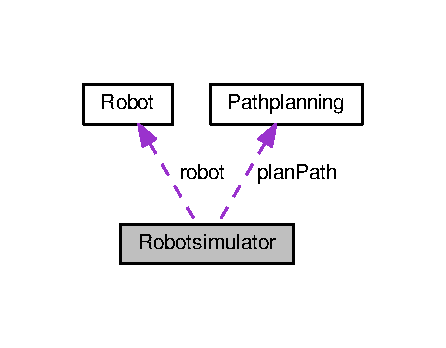
\includegraphics[width=214pt]{classRobotsimulator__coll__graph}
\end{center}
\end{figure}
\subsection*{Static Public Member Functions}
\begin{DoxyCompactItemize}
\item 
static int \hyperlink{classRobotsimulator_ab9d22fcac6da5b0c3806d015cdcd129d}{draw\+Outer\+Circle} (int centerx, int centery, int r)
\begin{DoxyCompactList}\small\item\em method to draw outer circle of joint \end{DoxyCompactList}\item 
static int \hyperlink{classRobotsimulator_a091403abfa76134b3135d98ea6fe24c4}{draw\+Inner\+Circle} (int centerx, int centery, int r)
\begin{DoxyCompactList}\small\item\em method to draw inner circle of joint \end{DoxyCompactList}\item 
static int \hyperlink{classRobotsimulator_a14ea782deab112fa6d3fc864a8aca2e8}{draw\+Joint} (int centerx, int centery)
\begin{DoxyCompactList}\small\item\em method to draw the joint using outercircle and innercircle methods \end{DoxyCompactList}\item 
static int \hyperlink{classRobotsimulator_a7b8564dcb925538dd55ec7d291d138dd}{draw\+Link\+Btn\+Joints} (float cx1, float cy1, float cx2, float cy2)
\begin{DoxyCompactList}\small\item\em method to draw link between joints \end{DoxyCompactList}\item 
static int {\bfseries draw\+End\+Effector} (float centerx, float centery)\hypertarget{classRobotsimulator_aabbda363024a68c3dc2050c20214a098}{}\label{classRobotsimulator_aabbda363024a68c3dc2050c20214a098}

\item 
static void \hyperlink{classRobotsimulator_a94348f09e5ce52444d4f0f526e723bc5}{display\+Arm} (void)
\begin{DoxyCompactList}\small\item\em method to display robot arm \end{DoxyCompactList}\item 
static void \hyperlink{classRobotsimulator_a24d1290882d5bac99e860fcf822fdc44}{reshape} (int w, int h)
\begin{DoxyCompactList}\small\item\em method to reshape the arm \end{DoxyCompactList}\item 
static void \hyperlink{classRobotsimulator_a9b1a52a2863af168184ab996858a764c}{display} (void)
\begin{DoxyCompactList}\small\item\em method to display all components for simulation \end{DoxyCompactList}\item 
static int \hyperlink{classRobotsimulator_aef4f47da29aede919802a5cc6e67fadb}{draw\+Path\+Circle} (void)
\begin{DoxyCompactList}\small\item\em method to draw Circular path taken by robot \end{DoxyCompactList}\item 
static int \hyperlink{classRobotsimulator_ab3f7118a0c8ee44dfc0e4d672e017b79}{draw\+Target} (float x, float y)
\begin{DoxyCompactList}\small\item\em method to draw Target point \end{DoxyCompactList}\item 
static void \hyperlink{classRobotsimulator_a96d2a360625f5b96b08ca0f8031c99f9}{run\+Simulation} (int argc, char $\ast$argv\mbox{[}$\,$\mbox{]})
\begin{DoxyCompactList}\small\item\em method to display all components for simulation \end{DoxyCompactList}\end{DoxyCompactItemize}
\subsection*{Static Public Attributes}
\begin{DoxyCompactItemize}
\item 
static \hyperlink{classRobot}{Robot} \hyperlink{classRobotsimulator_a7cc3a089ea219493264683338dd96b9d}{robot}\hypertarget{classRobotsimulator_a7cc3a089ea219493264683338dd96b9d}{}\label{classRobotsimulator_a7cc3a089ea219493264683338dd96b9d}

\begin{DoxyCompactList}\small\item\em static objects of \hyperlink{classRobot}{Robot} and \hyperlink{classPathplanning}{Pathplanning} class \end{DoxyCompactList}\item 
static \hyperlink{classPathplanning}{Pathplanning} {\bfseries plan\+Path}\hypertarget{classRobotsimulator_aa2a8d3f1b8c4bfbc4999bc4ebde3924a}{}\label{classRobotsimulator_aa2a8d3f1b8c4bfbc4999bc4ebde3924a}

\end{DoxyCompactItemize}


\subsection{Detailed Description}
declaration of \hyperlink{classRobotsimulator}{Robotsimulator} class 

\subsection{Member Function Documentation}
\index{Robotsimulator@{Robotsimulator}!display@{display}}
\index{display@{display}!Robotsimulator@{Robotsimulator}}
\subsubsection[{\texorpdfstring{display(void)}{display(void)}}]{\setlength{\rightskip}{0pt plus 5cm}void Robotsimulator\+::display (
\begin{DoxyParamCaption}
\item[{void}]{}
\end{DoxyParamCaption}
)\hspace{0.3cm}{\ttfamily [static]}}\hypertarget{classRobotsimulator_a9b1a52a2863af168184ab996858a764c}{}\label{classRobotsimulator_a9b1a52a2863af168184ab996858a764c}


method to display all components for simulation 


\begin{DoxyParams}{Parameters}
{\em void} & \\
\hline
\end{DoxyParams}
\begin{DoxyReturn}{Returns}
void -\/ displays components 
\end{DoxyReturn}
Method to set white background

display string \index{Robotsimulator@{Robotsimulator}!display\+Arm@{display\+Arm}}
\index{display\+Arm@{display\+Arm}!Robotsimulator@{Robotsimulator}}
\subsubsection[{\texorpdfstring{display\+Arm(void)}{displayArm(void)}}]{\setlength{\rightskip}{0pt plus 5cm}void Robotsimulator\+::display\+Arm (
\begin{DoxyParamCaption}
\item[{void}]{}
\end{DoxyParamCaption}
)\hspace{0.3cm}{\ttfamily [static]}}\hypertarget{classRobotsimulator_a94348f09e5ce52444d4f0f526e723bc5}{}\label{classRobotsimulator_a94348f09e5ce52444d4f0f526e723bc5}


method to display robot arm 


\begin{DoxyParams}{Parameters}
{\em void} & \\
\hline
\end{DoxyParams}
\begin{DoxyReturn}{Returns}
void 
\end{DoxyReturn}
update robots end\+Effector coordinates \index{Robotsimulator@{Robotsimulator}!draw\+Inner\+Circle@{draw\+Inner\+Circle}}
\index{draw\+Inner\+Circle@{draw\+Inner\+Circle}!Robotsimulator@{Robotsimulator}}
\subsubsection[{\texorpdfstring{draw\+Inner\+Circle(int centerx, int centery, int r)}{drawInnerCircle(int centerx, int centery, int r)}}]{\setlength{\rightskip}{0pt plus 5cm}int Robotsimulator\+::draw\+Inner\+Circle (
\begin{DoxyParamCaption}
\item[{int}]{centerx, }
\item[{int}]{centery, }
\item[{int}]{r}
\end{DoxyParamCaption}
)\hspace{0.3cm}{\ttfamily [static]}}\hypertarget{classRobotsimulator_a091403abfa76134b3135d98ea6fe24c4}{}\label{classRobotsimulator_a091403abfa76134b3135d98ea6fe24c4}


method to draw inner circle of joint 


\begin{DoxyParams}{Parameters}
{\em centerx} & -\/ x Coordinate of Joint\\
\hline
{\em centery} & -\/ y Coordinate of Joint\\
\hline
\end{DoxyParams}
\begin{DoxyReturn}{Returns}
int -\/ for testing purposes 
\end{DoxyReturn}
black foreground \index{Robotsimulator@{Robotsimulator}!draw\+Joint@{draw\+Joint}}
\index{draw\+Joint@{draw\+Joint}!Robotsimulator@{Robotsimulator}}
\subsubsection[{\texorpdfstring{draw\+Joint(int centerx, int centery)}{drawJoint(int centerx, int centery)}}]{\setlength{\rightskip}{0pt plus 5cm}int Robotsimulator\+::draw\+Joint (
\begin{DoxyParamCaption}
\item[{int}]{centerx, }
\item[{int}]{centery}
\end{DoxyParamCaption}
)\hspace{0.3cm}{\ttfamily [static]}}\hypertarget{classRobotsimulator_a14ea782deab112fa6d3fc864a8aca2e8}{}\label{classRobotsimulator_a14ea782deab112fa6d3fc864a8aca2e8}


method to draw the joint using outercircle and innercircle methods 


\begin{DoxyParams}{Parameters}
{\em centerx} & -\/ x Coordinate of Joint\\
\hline
{\em centery} & -\/ y Coordinate of Joint\\
\hline
\end{DoxyParams}
\begin{DoxyReturn}{Returns}
returns 1 to indicate success 
\end{DoxyReturn}
\index{Robotsimulator@{Robotsimulator}!draw\+Link\+Btn\+Joints@{draw\+Link\+Btn\+Joints}}
\index{draw\+Link\+Btn\+Joints@{draw\+Link\+Btn\+Joints}!Robotsimulator@{Robotsimulator}}
\subsubsection[{\texorpdfstring{draw\+Link\+Btn\+Joints(float cx1, float cy1, float cx2, float cy2)}{drawLinkBtnJoints(float cx1, float cy1, float cx2, float cy2)}}]{\setlength{\rightskip}{0pt plus 5cm}int Robotsimulator\+::draw\+Link\+Btn\+Joints (
\begin{DoxyParamCaption}
\item[{float}]{cx1, }
\item[{float}]{cy1, }
\item[{float}]{cx2, }
\item[{float}]{cy2}
\end{DoxyParamCaption}
)\hspace{0.3cm}{\ttfamily [static]}}\hypertarget{classRobotsimulator_a7b8564dcb925538dd55ec7d291d138dd}{}\label{classRobotsimulator_a7b8564dcb925538dd55ec7d291d138dd}


method to draw link between joints 


\begin{DoxyParams}{Parameters}
{\em cx1} & -\/ X coordinate of Joint1\\
\hline
{\em cy1} & -\/ Y coordinate of Joint1\\
\hline
{\em cx2} & -\/ X coordinate of Joint2\\
\hline
{\em cy2} & -\/ Y coordinate of joint2\\
\hline
\end{DoxyParams}
\begin{DoxyReturn}{Returns}
int -\/ returns 1 to indicate success 
\end{DoxyReturn}
\index{Robotsimulator@{Robotsimulator}!draw\+Outer\+Circle@{draw\+Outer\+Circle}}
\index{draw\+Outer\+Circle@{draw\+Outer\+Circle}!Robotsimulator@{Robotsimulator}}
\subsubsection[{\texorpdfstring{draw\+Outer\+Circle(int centerx, int centery, int r)}{drawOuterCircle(int centerx, int centery, int r)}}]{\setlength{\rightskip}{0pt plus 5cm}int Robotsimulator\+::draw\+Outer\+Circle (
\begin{DoxyParamCaption}
\item[{int}]{centerx, }
\item[{int}]{centery, }
\item[{int}]{r}
\end{DoxyParamCaption}
)\hspace{0.3cm}{\ttfamily [static]}}\hypertarget{classRobotsimulator_ab9d22fcac6da5b0c3806d015cdcd129d}{}\label{classRobotsimulator_ab9d22fcac6da5b0c3806d015cdcd129d}


method to draw outer circle of joint 


\begin{DoxyParams}{Parameters}
{\em centerx} & -\/ x Coordinate of Joint\\
\hline
{\em centery} & -\/ y Coordinate of Joint\\
\hline
\end{DoxyParams}
\begin{DoxyReturn}{Returns}
int -\/ for testing purposes 
\end{DoxyReturn}
black foreground \index{Robotsimulator@{Robotsimulator}!draw\+Path\+Circle@{draw\+Path\+Circle}}
\index{draw\+Path\+Circle@{draw\+Path\+Circle}!Robotsimulator@{Robotsimulator}}
\subsubsection[{\texorpdfstring{draw\+Path\+Circle(void)}{drawPathCircle(void)}}]{\setlength{\rightskip}{0pt plus 5cm}int Robotsimulator\+::draw\+Path\+Circle (
\begin{DoxyParamCaption}
\item[{void}]{}
\end{DoxyParamCaption}
)\hspace{0.3cm}{\ttfamily [static]}}\hypertarget{classRobotsimulator_aef4f47da29aede919802a5cc6e67fadb}{}\label{classRobotsimulator_aef4f47da29aede919802a5cc6e67fadb}


method to draw Circular path taken by robot 

\begin{DoxyReturn}{Returns}
returns 1 to indicate success 
\end{DoxyReturn}
black foreground \index{Robotsimulator@{Robotsimulator}!draw\+Target@{draw\+Target}}
\index{draw\+Target@{draw\+Target}!Robotsimulator@{Robotsimulator}}
\subsubsection[{\texorpdfstring{draw\+Target(float x, float y)}{drawTarget(float x, float y)}}]{\setlength{\rightskip}{0pt plus 5cm}int Robotsimulator\+::draw\+Target (
\begin{DoxyParamCaption}
\item[{float}]{x, }
\item[{float}]{y}
\end{DoxyParamCaption}
)\hspace{0.3cm}{\ttfamily [static]}}\hypertarget{classRobotsimulator_ab3f7118a0c8ee44dfc0e4d672e017b79}{}\label{classRobotsimulator_ab3f7118a0c8ee44dfc0e4d672e017b79}


method to draw Target point 


\begin{DoxyParams}{Parameters}
{\em x} & -\/ X coordinate of target point\\
\hline
{\em y} & -\/ Y coordinate of target point\\
\hline
\end{DoxyParams}
\begin{DoxyReturn}{Returns}
returns 1 to indicate success 
\end{DoxyReturn}
\index{Robotsimulator@{Robotsimulator}!reshape@{reshape}}
\index{reshape@{reshape}!Robotsimulator@{Robotsimulator}}
\subsubsection[{\texorpdfstring{reshape(int w, int h)}{reshape(int w, int h)}}]{\setlength{\rightskip}{0pt plus 5cm}void Robotsimulator\+::reshape (
\begin{DoxyParamCaption}
\item[{int}]{w, }
\item[{int}]{h}
\end{DoxyParamCaption}
)\hspace{0.3cm}{\ttfamily [static]}}\hypertarget{classRobotsimulator_a24d1290882d5bac99e860fcf822fdc44}{}\label{classRobotsimulator_a24d1290882d5bac99e860fcf822fdc44}


method to reshape the arm 


\begin{DoxyParams}{Parameters}
{\em } & \\
\hline
\end{DoxyParams}
Axis of window x axis from -\/50 to 50 y axis from -\/50 to 50 \index{Robotsimulator@{Robotsimulator}!run\+Simulation@{run\+Simulation}}
\index{run\+Simulation@{run\+Simulation}!Robotsimulator@{Robotsimulator}}
\subsubsection[{\texorpdfstring{run\+Simulation(int argc, char $\ast$argv[])}{runSimulation(int argc, char *argv[])}}]{\setlength{\rightskip}{0pt plus 5cm}void Robotsimulator\+::run\+Simulation (
\begin{DoxyParamCaption}
\item[{int}]{argc, }
\item[{char $\ast$}]{argv\mbox{[}$\,$\mbox{]}}
\end{DoxyParamCaption}
)\hspace{0.3cm}{\ttfamily [static]}}\hypertarget{classRobotsimulator_a96d2a360625f5b96b08ca0f8031c99f9}{}\label{classRobotsimulator_a96d2a360625f5b96b08ca0f8031c99f9}


method to display all components for simulation 

method to start simulation


\begin{DoxyParams}{Parameters}
{\em void} & \\
\hline
\end{DoxyParams}
\begin{DoxyReturn}{Returns}
void -\/ displays components
\end{DoxyReturn}

\begin{DoxyParams}{Parameters}
{\em command} & line arguments(\+Not used but needed for opengl library)\\
\hline
\end{DoxyParams}
\begin{DoxyReturn}{Returns}
void -\/ displays arm 
\end{DoxyReturn}
\hyperlink{classRobot}{Robot} functionalities to test

initialize window

callback functions calls the display function

calls the reshape function

calls timer function

Events are looped continuously 

The documentation for this class was generated from the following files\+:\begin{DoxyCompactItemize}
\item 
/home/eashwar/\+Desktop/\+E\+N\+P\+M808\+X\+\_\+\+M\+I\+D\+T\+E\+R\+M/include/\hyperlink{Robotsimulator_8hpp}{Robotsimulator.\+hpp}\item 
/home/eashwar/\+Desktop/\+E\+N\+P\+M808\+X\+\_\+\+M\+I\+D\+T\+E\+R\+M/app/\hyperlink{Robotsimulator_8cpp}{Robotsimulator.\+cpp}\end{DoxyCompactItemize}

\chapter{File Documentation}
\hypertarget{Pathplanning_8cpp}{}\section{/home/eashwar/\+Desktop/\+E\+N\+P\+M808\+X\+\_\+\+M\+I\+D\+T\+E\+R\+M/app/\+Pathplanning.cpp File Reference}
\label{Pathplanning_8cpp}\index{/home/eashwar/\+Desktop/\+E\+N\+P\+M808\+X\+\_\+\+M\+I\+D\+T\+E\+R\+M/app/\+Pathplanning.\+cpp@{/home/eashwar/\+Desktop/\+E\+N\+P\+M808\+X\+\_\+\+M\+I\+D\+T\+E\+R\+M/app/\+Pathplanning.\+cpp}}


cpp program for definition and implementation of the methods of \hyperlink{classPathplanning}{Pathplanning} class  


{\ttfamily \#include \char`\"{}Pathplanning.\+hpp\char`\"{}}\\*
Include dependency graph for Pathplanning.\+cpp\+:
\nopagebreak
\begin{figure}[H]
\begin{center}
\leavevmode
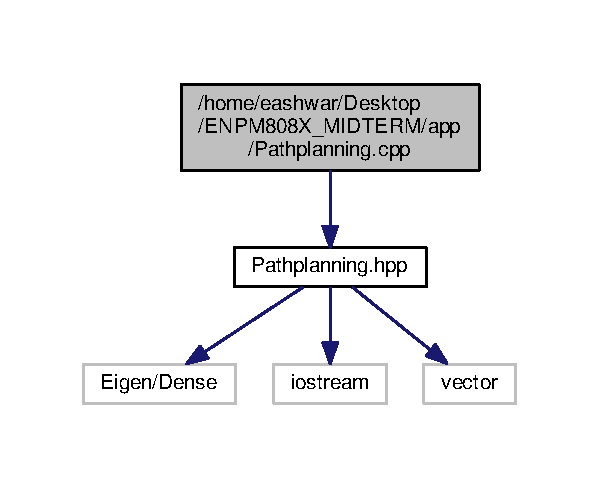
\includegraphics[width=288pt]{Pathplanning_8cpp__incl}
\end{center}
\end{figure}


\subsection{Detailed Description}
cpp program for definition and implementation of the methods of \hyperlink{classPathplanning}{Pathplanning} class 

\begin{DoxyAuthor}{Author}
Akwasi A Obeng(\+Driver) Eashwar Sathyamurthy(\+Navigator)
\end{DoxyAuthor}
\begin{DoxyVersion}{Version}
1
\end{DoxyVersion}
\begin{DoxyDate}{Date}
2019-\/10-\/12
\end{DoxyDate}
This program implements the methods of the \hyperlink{classPathplanning}{Pathplanning} class from \hyperlink{Pathplanning_8hpp}{Pathplanning.\+hpp} header file 
\hypertarget{Robot_8cpp}{}\section{/home/eashwar/\+Desktop/\+E\+N\+P\+M808\+X\+\_\+\+M\+I\+D\+T\+E\+R\+M/app/\+Robot.cpp File Reference}
\label{Robot_8cpp}\index{/home/eashwar/\+Desktop/\+E\+N\+P\+M808\+X\+\_\+\+M\+I\+D\+T\+E\+R\+M/app/\+Robot.\+cpp@{/home/eashwar/\+Desktop/\+E\+N\+P\+M808\+X\+\_\+\+M\+I\+D\+T\+E\+R\+M/app/\+Robot.\+cpp}}


cpp program for definition and implementation of the methods of \hyperlink{classRobot}{Robot} class  


{\ttfamily \#include \char`\"{}Robot.\+hpp\char`\"{}}\\*
Include dependency graph for Robot.\+cpp\+:
\nopagebreak
\begin{figure}[H]
\begin{center}
\leavevmode
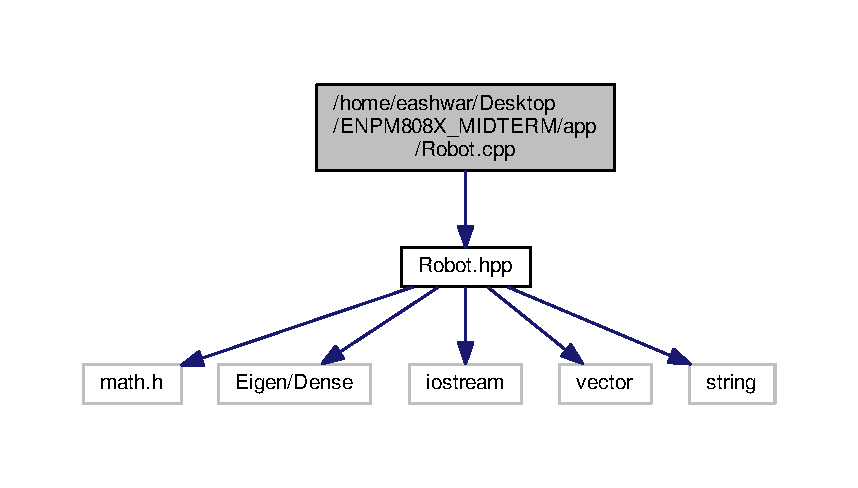
\includegraphics[width=350pt]{Robot_8cpp__incl}
\end{center}
\end{figure}


\subsection{Detailed Description}
cpp program for definition and implementation of the methods of \hyperlink{classRobot}{Robot} class 

\begin{DoxyAuthor}{Author}
Eashwar Sathyamurthy(\+Driver) Akwasi A Obeng(\+Navigator)
\end{DoxyAuthor}
\begin{DoxyVersion}{Version}
1
\end{DoxyVersion}
\begin{DoxyDate}{Date}
2019-\/10-\/12
\end{DoxyDate}
This program implements the methods of the \hyperlink{classRobot}{Robot} class from \hyperlink{Robot_8hpp}{Robot.\+hpp} header file 
\hypertarget{Robotsimulator_8cpp}{}\section{/home/eashwar/\+Desktop/\+E\+N\+P\+M808\+X\+\_\+\+M\+I\+D\+T\+E\+R\+M/app/\+Robotsimulator.cpp File Reference}
\label{Robotsimulator_8cpp}\index{/home/eashwar/\+Desktop/\+E\+N\+P\+M808\+X\+\_\+\+M\+I\+D\+T\+E\+R\+M/app/\+Robotsimulator.\+cpp@{/home/eashwar/\+Desktop/\+E\+N\+P\+M808\+X\+\_\+\+M\+I\+D\+T\+E\+R\+M/app/\+Robotsimulator.\+cpp}}


cpp program for definition and implementation of the methods of \hyperlink{classRobotsimulator}{Robotsimulator} class  


{\ttfamily \#include \char`\"{}Robotsimulator.\+hpp\char`\"{}}\\*
Include dependency graph for Robotsimulator.\+cpp\+:
\nopagebreak
\begin{figure}[H]
\begin{center}
\leavevmode
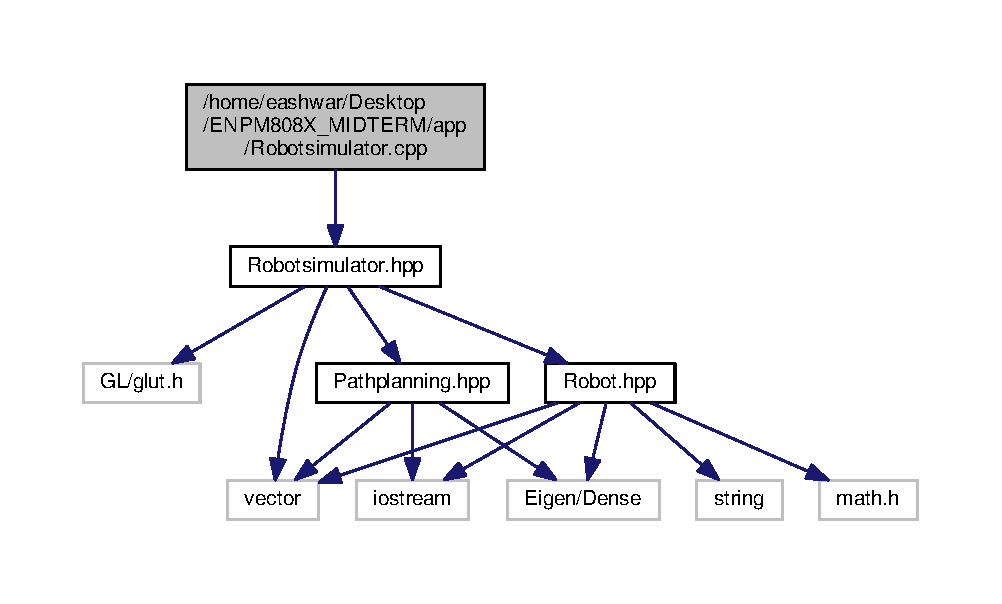
\includegraphics[width=350pt]{Robotsimulator_8cpp__incl}
\end{center}
\end{figure}
\subsection*{Functions}
\begin{DoxyCompactItemize}
\item 
Eigen\+::\+Vector2f {\bfseries joint1} (0, 0)\hypertarget{Robotsimulator_8cpp_ae97978fcc262bd4f84ae1176ccaea736}{}\label{Robotsimulator_8cpp_ae97978fcc262bd4f84ae1176ccaea736}

\item 
Eigen\+::\+Vector2f {\bfseries joint2} (20, 0)\hypertarget{Robotsimulator_8cpp_a9b885fdd3c55a5cf19777110175986af}{}\label{Robotsimulator_8cpp_a9b885fdd3c55a5cf19777110175986af}

\item 
Eigen\+::\+Vector2f {\bfseries end\+Effector} (40, 0)\hypertarget{Robotsimulator_8cpp_a34ee21b9d16dca3cb755749f05e444fd}{}\label{Robotsimulator_8cpp_a34ee21b9d16dca3cb755749f05e444fd}

\item 
Eigen\+::\+Vector2d {\bfseries path} (1,-\/1)\hypertarget{Robotsimulator_8cpp_af327f93222ca6bc0e610c15cc3eef7d9}{}\label{Robotsimulator_8cpp_af327f93222ca6bc0e610c15cc3eef7d9}

\item 
Eigen\+::\+Vector2d {\bfseries angles} (1, 1)\hypertarget{Robotsimulator_8cpp_a7af6d0c01fe04fe335c000242eab3cba}{}\label{Robotsimulator_8cpp_a7af6d0c01fe04fe335c000242eab3cba}

\item 
void \hyperlink{Robotsimulator_8cpp_a60ebef228b6633754a3122edd12a5473}{timer} (int)
\begin{DoxyCompactList}\small\item\em method times the display \end{DoxyCompactList}\end{DoxyCompactItemize}
\subsection*{Variables}
\begin{DoxyCompactItemize}
\item 
Eigen\+::\+Vector2f {\bfseries end\+Effector\+Copy} = end\+Effector\hypertarget{Robotsimulator_8cpp_a76b40015715e78eb1c6486d9ec73a40b}{}\label{Robotsimulator_8cpp_a76b40015715e78eb1c6486d9ec73a40b}

\item 
float {\bfseries targetX}\hypertarget{Robotsimulator_8cpp_a5516cb7e2fddc92ffa1e3668e4250079}{}\label{Robotsimulator_8cpp_a5516cb7e2fddc92ffa1e3668e4250079}

\item 
float {\bfseries targetY}\hypertarget{Robotsimulator_8cpp_a0dbd9a3242235c41e946bd75fda94572}{}\label{Robotsimulator_8cpp_a0dbd9a3242235c41e946bd75fda94572}

\item 
int {\bfseries display\+Type}\hypertarget{Robotsimulator_8cpp_aafe478357364a961cc3cddf85a8f626e}{}\label{Robotsimulator_8cpp_aafe478357364a961cc3cddf85a8f626e}

\end{DoxyCompactItemize}


\subsection{Detailed Description}
cpp program for definition and implementation of the methods of \hyperlink{classRobotsimulator}{Robotsimulator} class 

\begin{DoxyAuthor}{Author}
Akwasi A Obeng(\+Driver) Eashwar Sathyamurthy(\+Navigator)
\end{DoxyAuthor}
\begin{DoxyVersion}{Version}
1
\end{DoxyVersion}
\begin{DoxyDate}{Date}
2019-\/10-\/12
\end{DoxyDate}
This program implements the methods of the \hyperlink{classRobotsimulator}{Robotsimulator} class from \hyperlink{Robotsimulator_8hpp}{Robotsimulator.\+hpp} header file 

\subsection{Function Documentation}
\index{Robotsimulator.\+cpp@{Robotsimulator.\+cpp}!timer@{timer}}
\index{timer@{timer}!Robotsimulator.\+cpp@{Robotsimulator.\+cpp}}
\subsubsection[{\texorpdfstring{timer(int)}{timer(int)}}]{\setlength{\rightskip}{0pt plus 5cm}void timer (
\begin{DoxyParamCaption}
\item[{int}]{}
\end{DoxyParamCaption}
)}\hypertarget{Robotsimulator_8cpp_a60ebef228b6633754a3122edd12a5473}{}\label{Robotsimulator_8cpp_a60ebef228b6633754a3122edd12a5473}


method times the display 


\begin{DoxyParams}{Parameters}
{\em Referesh} & rate for display\\
\hline
\end{DoxyParams}
\begin{DoxyReturn}{Returns}
void 
\end{DoxyReturn}
displays 60frames in 1000 milliseconds 
\hypertarget{Pathplanning_8hpp}{}\section{/home/eashwar/\+Desktop/\+E\+N\+P\+M808\+X\+\_\+\+M\+I\+D\+T\+E\+R\+M/include/\+Pathplanning.hpp File Reference}
\label{Pathplanning_8hpp}\index{/home/eashwar/\+Desktop/\+E\+N\+P\+M808\+X\+\_\+\+M\+I\+D\+T\+E\+R\+M/include/\+Pathplanning.\+hpp@{/home/eashwar/\+Desktop/\+E\+N\+P\+M808\+X\+\_\+\+M\+I\+D\+T\+E\+R\+M/include/\+Pathplanning.\+hpp}}


declaration for \hyperlink{classPathplanning}{Pathplanning} class  


{\ttfamily \#include $<$Eigen/\+Dense$>$}\\*
{\ttfamily \#include $<$iostream$>$}\\*
{\ttfamily \#include $<$vector$>$}\\*
Include dependency graph for Pathplanning.\+hpp\+:
\nopagebreak
\begin{figure}[H]
\begin{center}
\leavevmode
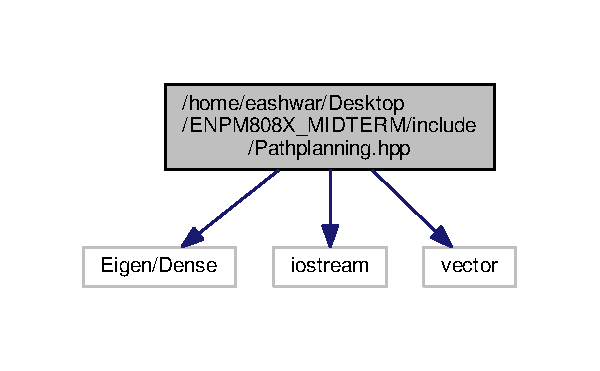
\includegraphics[width=288pt]{Pathplanning_8hpp__incl}
\end{center}
\end{figure}
This graph shows which files directly or indirectly include this file\+:
\nopagebreak
\begin{figure}[H]
\begin{center}
\leavevmode
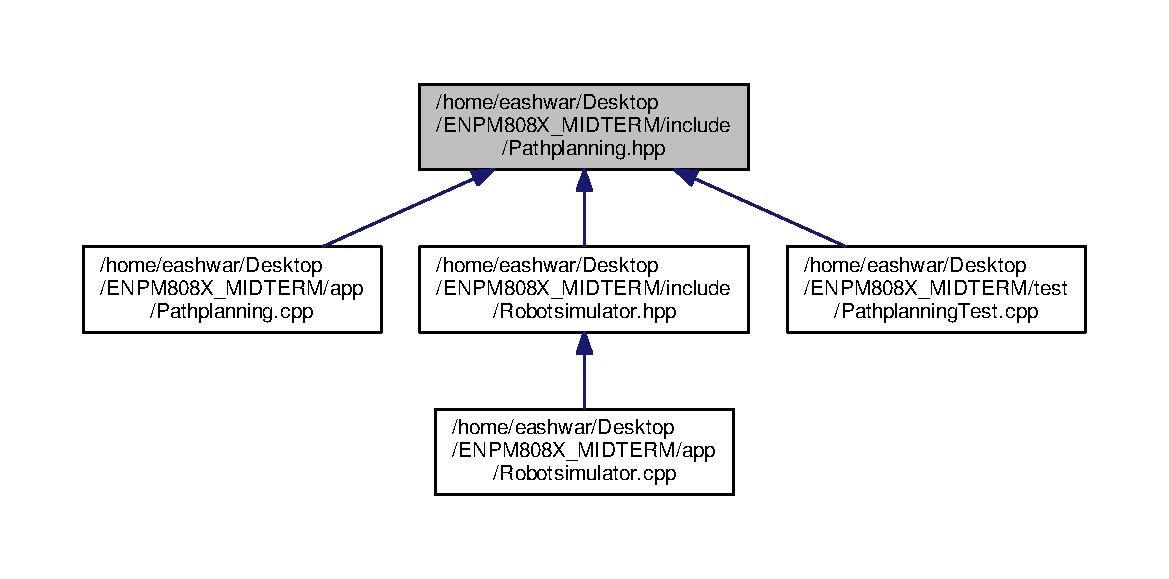
\includegraphics[width=350pt]{Pathplanning_8hpp__dep__incl}
\end{center}
\end{figure}
\subsection*{Classes}
\begin{DoxyCompactItemize}
\item 
class \hyperlink{classPathplanning}{Pathplanning}
\begin{DoxyCompactList}\small\item\em declaration of \hyperlink{classPathplanning}{Pathplanning} class \end{DoxyCompactList}\end{DoxyCompactItemize}
\subsection*{Macros}
\begin{DoxyCompactItemize}
\item 
\#define {\bfseries PI}~3.\+1415926\hypertarget{Pathplanning_8hpp_a598a3330b3c21701223ee0ca14316eca}{}\label{Pathplanning_8hpp_a598a3330b3c21701223ee0ca14316eca}

\end{DoxyCompactItemize}


\subsection{Detailed Description}
declaration for \hyperlink{classPathplanning}{Pathplanning} class 

\begin{DoxyAuthor}{Author}
Akwasi A Obeng(\+Driver) Eashwar Sathyamurthy(\+Navigator)
\end{DoxyAuthor}
\begin{DoxyVersion}{Version}
1
\end{DoxyVersion}
\begin{DoxyDate}{Date}
2019-\/10-\/12
\end{DoxyDate}
This .hpp file has declarations for the class attributes and methods for simple functionality of path planning of robot arm mainpulator. 
\hypertarget{Robot_8hpp}{}\section{/home/eashwar/\+Desktop/\+E\+N\+P\+M808\+X\+\_\+\+M\+I\+D\+T\+E\+R\+M/include/\+Robot.hpp File Reference}
\label{Robot_8hpp}\index{/home/eashwar/\+Desktop/\+E\+N\+P\+M808\+X\+\_\+\+M\+I\+D\+T\+E\+R\+M/include/\+Robot.\+hpp@{/home/eashwar/\+Desktop/\+E\+N\+P\+M808\+X\+\_\+\+M\+I\+D\+T\+E\+R\+M/include/\+Robot.\+hpp}}


declaration for \hyperlink{classRobot}{Robot} class  


{\ttfamily \#include $<$math.\+h$>$}\\*
{\ttfamily \#include $<$Eigen/\+Dense$>$}\\*
{\ttfamily \#include $<$iostream$>$}\\*
{\ttfamily \#include $<$vector$>$}\\*
{\ttfamily \#include $<$string$>$}\\*
Include dependency graph for Robot.\+hpp\+:
\nopagebreak
\begin{figure}[H]
\begin{center}
\leavevmode
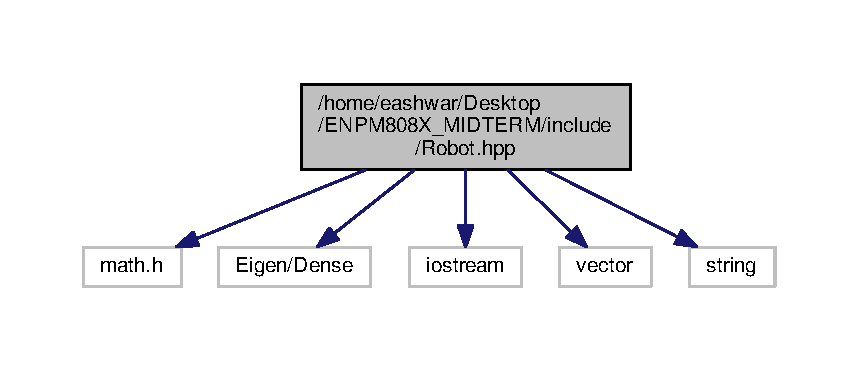
\includegraphics[width=350pt]{Robot_8hpp__incl}
\end{center}
\end{figure}
This graph shows which files directly or indirectly include this file\+:
\nopagebreak
\begin{figure}[H]
\begin{center}
\leavevmode
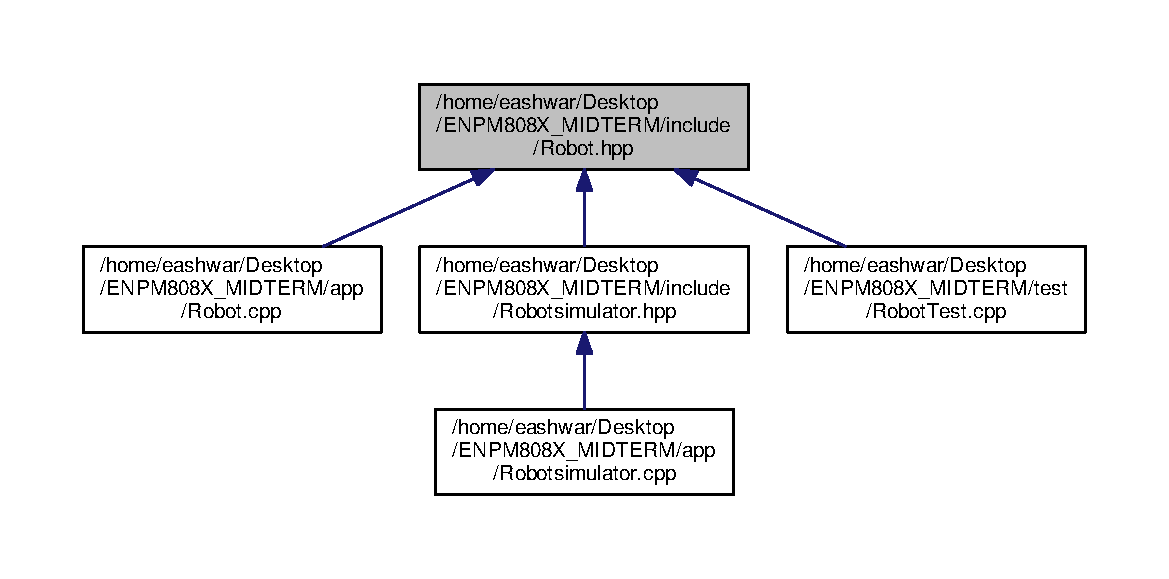
\includegraphics[width=350pt]{Robot_8hpp__dep__incl}
\end{center}
\end{figure}
\subsection*{Classes}
\begin{DoxyCompactItemize}
\item 
class \hyperlink{classRobot}{Robot}
\begin{DoxyCompactList}\small\item\em declaration of \hyperlink{classRobot}{Robot} class \end{DoxyCompactList}\end{DoxyCompactItemize}


\subsection{Detailed Description}
declaration for \hyperlink{classRobot}{Robot} class 

\begin{DoxyAuthor}{Author}
Eashwar Sathyamurthy(\+Driver) Akwasi A Obeng(\+Navigator)//
\end{DoxyAuthor}
\begin{DoxyVersion}{Version}
1
\end{DoxyVersion}
\begin{DoxyDate}{Date}
2019-\/10-\/12
\end{DoxyDate}
This .hpp file has declarations for the class attributes and methods for simple functionality of the robot arm mainpulator. 
\hypertarget{Robotsimulator_8hpp}{}\section{/home/eashwar/\+Desktop/\+E\+N\+P\+M808\+X\+\_\+\+M\+I\+D\+T\+E\+R\+M/include/\+Robotsimulator.hpp File Reference}
\label{Robotsimulator_8hpp}\index{/home/eashwar/\+Desktop/\+E\+N\+P\+M808\+X\+\_\+\+M\+I\+D\+T\+E\+R\+M/include/\+Robotsimulator.\+hpp@{/home/eashwar/\+Desktop/\+E\+N\+P\+M808\+X\+\_\+\+M\+I\+D\+T\+E\+R\+M/include/\+Robotsimulator.\+hpp}}


declaration for \hyperlink{classRobotsimulator}{Robotsimulator} class  


{\ttfamily \#include $<$G\+L/glut.\+h$>$}\\*
{\ttfamily \#include $<$vector$>$}\\*
{\ttfamily \#include \char`\"{}Pathplanning.\+hpp\char`\"{}}\\*
{\ttfamily \#include \char`\"{}Robot.\+hpp\char`\"{}}\\*
Include dependency graph for Robotsimulator.\+hpp\+:
\nopagebreak
\begin{figure}[H]
\begin{center}
\leavevmode
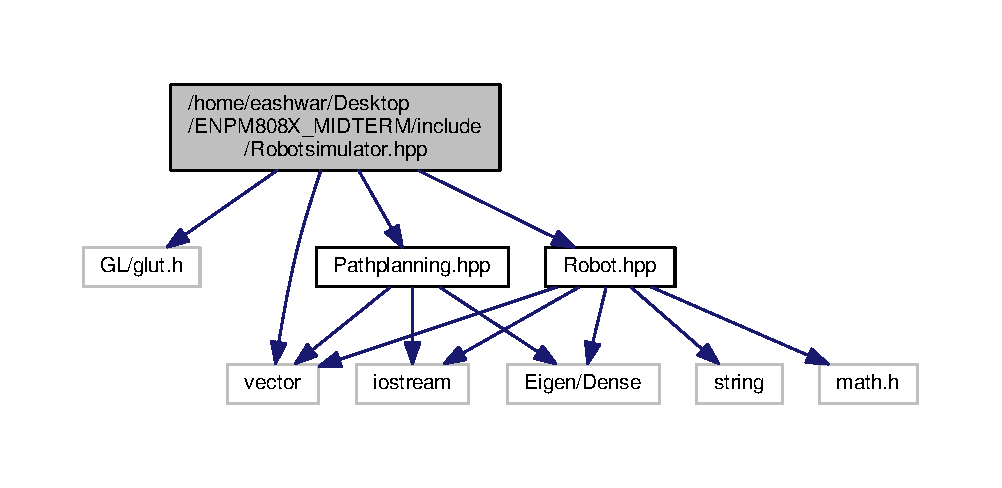
\includegraphics[width=350pt]{Robotsimulator_8hpp__incl}
\end{center}
\end{figure}
This graph shows which files directly or indirectly include this file\+:
\nopagebreak
\begin{figure}[H]
\begin{center}
\leavevmode
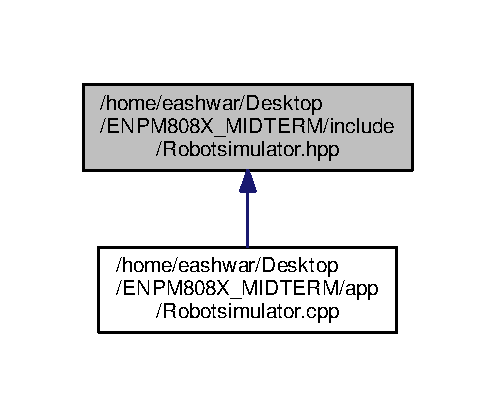
\includegraphics[width=238pt]{Robotsimulator_8hpp__dep__incl}
\end{center}
\end{figure}
\subsection*{Classes}
\begin{DoxyCompactItemize}
\item 
class \hyperlink{classRobotsimulator}{Robotsimulator}
\begin{DoxyCompactList}\small\item\em declaration of \hyperlink{classRobotsimulator}{Robotsimulator} class \end{DoxyCompactList}\end{DoxyCompactItemize}
\subsection*{Macros}
\begin{DoxyCompactItemize}
\item 
\#define {\bfseries PI}~3.\+1415926\hypertarget{Robotsimulator_8hpp_a598a3330b3c21701223ee0ca14316eca}{}\label{Robotsimulator_8hpp_a598a3330b3c21701223ee0ca14316eca}

\end{DoxyCompactItemize}


\subsection{Detailed Description}
declaration for \hyperlink{classRobotsimulator}{Robotsimulator} class 

\begin{DoxyAuthor}{Author}
Akwasi A Obeng(\+Driver) Eashwar Sathyamurthy(\+Navigator)
\end{DoxyAuthor}
\begin{DoxyVersion}{Version}
1
\end{DoxyVersion}
\begin{DoxyDate}{Date}
2019-\/10-\/12
\end{DoxyDate}
This .hpp file has declarations for the class attributes and methods for simple functionality of the robot arm mainpulator. 
\hypertarget{PathplanningTest_8cpp}{}\section{/home/eashwar/\+Desktop/\+E\+N\+P\+M808\+X\+\_\+\+M\+I\+D\+T\+E\+R\+M/test/\+Pathplanning\+Test.cpp File Reference}
\label{PathplanningTest_8cpp}\index{/home/eashwar/\+Desktop/\+E\+N\+P\+M808\+X\+\_\+\+M\+I\+D\+T\+E\+R\+M/test/\+Pathplanning\+Test.\+cpp@{/home/eashwar/\+Desktop/\+E\+N\+P\+M808\+X\+\_\+\+M\+I\+D\+T\+E\+R\+M/test/\+Pathplanning\+Test.\+cpp}}


test cases (Google Test framework) for \hyperlink{classPathplanning}{Pathplanning} class  


{\ttfamily \#include $<$gtest/gtest.\+h$>$}\\*
{\ttfamily \#include $<$iostream$>$}\\*
{\ttfamily \#include \char`\"{}Pathplanning.\+hpp\char`\"{}}\\*
Include dependency graph for Pathplanning\+Test.\+cpp\+:
\nopagebreak
\begin{figure}[H]
\begin{center}
\leavevmode
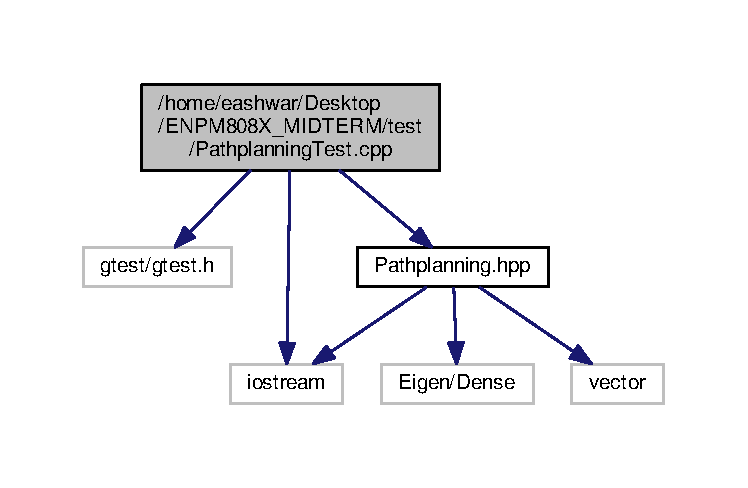
\includegraphics[width=350pt]{PathplanningTest_8cpp__incl}
\end{center}
\end{figure}
\subsection*{Functions}
\begin{DoxyCompactItemize}
\item 
\hyperlink{PathplanningTest_8cpp_a0589da1a834617e0c67033b00850bb82}{T\+E\+ST} (\hyperlink{classPathplanning}{Pathplanning}, Angles\+For\+Linear\+Path\+Method\+Testing)
\begin{DoxyCompactList}\small\item\em Unit Test for testing Angles\+For\+Linear\+Path method. \end{DoxyCompactList}\item 
\hyperlink{PathplanningTest_8cpp_a088c36743f52a3b1ac9f1f08b5adc968}{T\+E\+ST} (\hyperlink{classPathplanning}{Pathplanning}, Angles\+For\+Continuous\+Path\+Method\+Testing)
\begin{DoxyCompactList}\small\item\em Unit Test for testing Angles\+For\+Continuous\+Path method. \end{DoxyCompactList}\item 
\hyperlink{PathplanningTest_8cpp_ac73d9dded3c27ef1a1aa3b56646f4559}{T\+E\+ST} (\hyperlink{classPathplanning}{Pathplanning}, Angles\+For\+Circular\+Path\+Method\+Testing)
\begin{DoxyCompactList}\small\item\em Unit Test for testing Angles\+For\+Circular\+Path method. \end{DoxyCompactList}\end{DoxyCompactItemize}


\subsection{Detailed Description}
test cases (Google Test framework) for \hyperlink{classPathplanning}{Pathplanning} class 

test cases (Google Test framework) for \hyperlink{classRobotsimulator}{Robotsimulator} class

\begin{DoxyAuthor}{Author}
Part1\+: Eashwar Sathyamurthy(\+Driver) Akwasi A Obeng(\+Navigator)
\end{DoxyAuthor}
\begin{DoxyVersion}{Version}
1
\end{DoxyVersion}
\begin{DoxyDate}{Date}
2019-\/10-\/12
\end{DoxyDate}
This .cpp file has test cases definitions for the class methods of \hyperlink{classPathplanning}{Pathplanning} class

\begin{DoxyAuthor}{Author}
Part1\+: Eashwar Sathyamurthy(\+Driver) Akwasi A Obeng(\+Navigator)
\end{DoxyAuthor}
\begin{DoxyVersion}{Version}
1
\end{DoxyVersion}
\begin{DoxyDate}{Date}
2019-\/10-\/12
\end{DoxyDate}
This .cpp file has test cases definitions for the class methods of \hyperlink{classRobotsimulator}{Robotsimulator} class 

\subsection{Function Documentation}
\index{Pathplanning\+Test.\+cpp@{Pathplanning\+Test.\+cpp}!T\+E\+ST@{T\+E\+ST}}
\index{T\+E\+ST@{T\+E\+ST}!Pathplanning\+Test.\+cpp@{Pathplanning\+Test.\+cpp}}
\subsubsection[{\texorpdfstring{T\+E\+S\+T(\+Pathplanning, Angles\+For\+Linear\+Path\+Method\+Testing)}{TEST(Pathplanning, AnglesForLinearPathMethodTesting)}}]{\setlength{\rightskip}{0pt plus 5cm}T\+E\+ST (
\begin{DoxyParamCaption}
\item[{{\bf Pathplanning}}]{, }
\item[{Angles\+For\+Linear\+Path\+Method\+Testing}]{}
\end{DoxyParamCaption}
)}\hypertarget{PathplanningTest_8cpp_a0589da1a834617e0c67033b00850bb82}{}\label{PathplanningTest_8cpp_a0589da1a834617e0c67033b00850bb82}


Unit Test for testing Angles\+For\+Linear\+Path method. 

This test checks if the return value of the method is same the Eigen\+::\+Vector2d angles \index{Pathplanning\+Test.\+cpp@{Pathplanning\+Test.\+cpp}!T\+E\+ST@{T\+E\+ST}}
\index{T\+E\+ST@{T\+E\+ST}!Pathplanning\+Test.\+cpp@{Pathplanning\+Test.\+cpp}}
\subsubsection[{\texorpdfstring{T\+E\+S\+T(\+Pathplanning, Angles\+For\+Continuous\+Path\+Method\+Testing)}{TEST(Pathplanning, AnglesForContinuousPathMethodTesting)}}]{\setlength{\rightskip}{0pt plus 5cm}T\+E\+ST (
\begin{DoxyParamCaption}
\item[{{\bf Pathplanning}}]{, }
\item[{Angles\+For\+Continuous\+Path\+Method\+Testing}]{}
\end{DoxyParamCaption}
)}\hypertarget{PathplanningTest_8cpp_a088c36743f52a3b1ac9f1f08b5adc968}{}\label{PathplanningTest_8cpp_a088c36743f52a3b1ac9f1f08b5adc968}


Unit Test for testing Angles\+For\+Continuous\+Path method. 

This test checks if the return value of the method is same the Eigen\+::\+Vector2d angles \index{Pathplanning\+Test.\+cpp@{Pathplanning\+Test.\+cpp}!T\+E\+ST@{T\+E\+ST}}
\index{T\+E\+ST@{T\+E\+ST}!Pathplanning\+Test.\+cpp@{Pathplanning\+Test.\+cpp}}
\subsubsection[{\texorpdfstring{T\+E\+S\+T(\+Pathplanning, Angles\+For\+Circular\+Path\+Method\+Testing)}{TEST(Pathplanning, AnglesForCircularPathMethodTesting)}}]{\setlength{\rightskip}{0pt plus 5cm}T\+E\+ST (
\begin{DoxyParamCaption}
\item[{{\bf Pathplanning}}]{, }
\item[{Angles\+For\+Circular\+Path\+Method\+Testing}]{}
\end{DoxyParamCaption}
)}\hypertarget{PathplanningTest_8cpp_ac73d9dded3c27ef1a1aa3b56646f4559}{}\label{PathplanningTest_8cpp_ac73d9dded3c27ef1a1aa3b56646f4559}


Unit Test for testing Angles\+For\+Circular\+Path method. 

This test checks if the return value of the method is same the Eigen\+::\+Vector2d angles 
\hypertarget{RobotTest_8cpp}{}\section{/home/eashwar/\+Desktop/\+E\+N\+P\+M808\+X\+\_\+\+M\+I\+D\+T\+E\+R\+M/test/\+Robot\+Test.cpp File Reference}
\label{RobotTest_8cpp}\index{/home/eashwar/\+Desktop/\+E\+N\+P\+M808\+X\+\_\+\+M\+I\+D\+T\+E\+R\+M/test/\+Robot\+Test.\+cpp@{/home/eashwar/\+Desktop/\+E\+N\+P\+M808\+X\+\_\+\+M\+I\+D\+T\+E\+R\+M/test/\+Robot\+Test.\+cpp}}


test cases (Google Test framework) for \hyperlink{classRobot}{Robot} class  


{\ttfamily \#include $<$gtest/gtest.\+h$>$}\\*
{\ttfamily \#include $<$iostream$>$}\\*
{\ttfamily \#include \char`\"{}Robot.\+hpp\char`\"{}}\\*
Include dependency graph for Robot\+Test.\+cpp\+:
\nopagebreak
\begin{figure}[H]
\begin{center}
\leavevmode
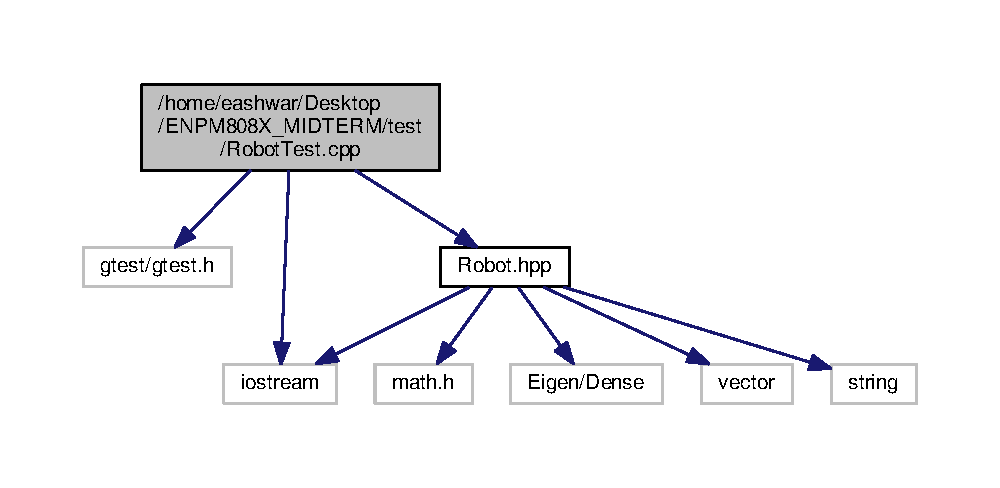
\includegraphics[width=350pt]{RobotTest_8cpp__incl}
\end{center}
\end{figure}
\subsection*{Functions}
\begin{DoxyCompactItemize}
\item 
\hyperlink{RobotTest_8cpp_a11f5fd481cbf51fdeaabcf6676ddda65}{T\+E\+ST} (\hyperlink{classRobot}{Robot}, testis\+In\+Workspace\+Method)
\begin{DoxyCompactList}\small\item\em Unit Test for testing is\+In\+Workspace(double,double) and rotate\+Robot(double,double) method. \end{DoxyCompactList}\item 
\hyperlink{RobotTest_8cpp_a42716e510826864dfde8defc81e7193c}{T\+E\+ST} (\hyperlink{classRobot}{Robot}, testtarget\+Reached\+Method)
\begin{DoxyCompactList}\small\item\em Unit Test for testing is\+In\+Workspace(double,double) and rotate\+Robot(double,double) method. \end{DoxyCompactList}\end{DoxyCompactItemize}


\subsection{Detailed Description}
test cases (Google Test framework) for \hyperlink{classRobot}{Robot} class 

\begin{DoxyAuthor}{Author}
Part1\+: Eashwar Sathyamurthy(\+Driver) Akwasi A Obeng(\+Navigator)
\end{DoxyAuthor}
\begin{DoxyVersion}{Version}
1
\end{DoxyVersion}
\begin{DoxyDate}{Date}
2019-\/10-\/12
\end{DoxyDate}
This .cpp file has test cases definitions for the class methods of \hyperlink{classRobot}{Robot} class 

\subsection{Function Documentation}
\index{Robot\+Test.\+cpp@{Robot\+Test.\+cpp}!T\+E\+ST@{T\+E\+ST}}
\index{T\+E\+ST@{T\+E\+ST}!Robot\+Test.\+cpp@{Robot\+Test.\+cpp}}
\subsubsection[{\texorpdfstring{T\+E\+S\+T(\+Robot, testis\+In\+Workspace\+Method)}{TEST(Robot, testisInWorkspaceMethod)}}]{\setlength{\rightskip}{0pt plus 5cm}T\+E\+ST (
\begin{DoxyParamCaption}
\item[{{\bf Robot}}]{, }
\item[{testis\+In\+Workspace\+Method}]{}
\end{DoxyParamCaption}
)}\hypertarget{RobotTest_8cpp_a11f5fd481cbf51fdeaabcf6676ddda65}{}\label{RobotTest_8cpp_a11f5fd481cbf51fdeaabcf6676ddda65}


Unit Test for testing is\+In\+Workspace(double,double) and rotate\+Robot(double,double) method. 

This test checks if the return value of the is\+In\+Workspace(double,double) method is true or false This test checks if the return value of the target\+Reached(double,double) method returns true or false to see if the target is reached or not. \index{Robot\+Test.\+cpp@{Robot\+Test.\+cpp}!T\+E\+ST@{T\+E\+ST}}
\index{T\+E\+ST@{T\+E\+ST}!Robot\+Test.\+cpp@{Robot\+Test.\+cpp}}
\subsubsection[{\texorpdfstring{T\+E\+S\+T(\+Robot, testtarget\+Reached\+Method)}{TEST(Robot, testtargetReachedMethod)}}]{\setlength{\rightskip}{0pt plus 5cm}T\+E\+ST (
\begin{DoxyParamCaption}
\item[{{\bf Robot}}]{, }
\item[{testtarget\+Reached\+Method}]{}
\end{DoxyParamCaption}
)}\hypertarget{RobotTest_8cpp_a42716e510826864dfde8defc81e7193c}{}\label{RobotTest_8cpp_a42716e510826864dfde8defc81e7193c}


Unit Test for testing is\+In\+Workspace(double,double) and rotate\+Robot(double,double) method. 

This test checks if the return value of the target\+Reached(double,double) method returns true or false to see if the target is reached or not. 
%--- End generated contents ---

% Index
\backmatter
\newpage
\phantomsection
\clearemptydoublepage
\addcontentsline{toc}{chapter}{Index}
\printindex

\end{document}
